\documentclass[11pt]{article}
\usepackage[margin=1in]{geometry}
\usepackage[T1]{fontenc}
\usepackage{lmodern}
\usepackage{amsmath,amssymb}
\usepackage{enumitem}
\usepackage{booktabs}
\usepackage{tikz}
\usetikzlibrary{arrows.meta,positioning}
\usepackage[colorlinks=true,urlcolor=blue,linkcolor=blue]{hyperref}
\setlist{nosep,leftmargin=*}

\title{Predicting ICLR 2025 Peer-Review Decisions with Bayesian Models}
\author{CSE 5825 Bayesian Machine Learning --- Jiazheng Li}
\date{September 2026}

\begin{document}
\maketitle

\section*{Research question and data}
Can information in peer reviews predict whether an ICLR 2025 submission is rejected or accepted as a poster, spotlight, or oral presentation? More specifically, do reviewer disagreement, changes after author rebuttal, and discussion participation contain information beyond the mean review rating?

The proposed dataset combines two public, OpenReview-derived releases for ICLR 2025. The \href{https://github.com/papercopilot/iclr-insights}{ICLR Insights score-change data} identify each paper by its OpenReview ID and provide each reviewer's initial and post-rebuttal rating, confidence, and other rubric scores. The corresponding \href{https://github.com/papercopilot/openreview}{Paper Copilot OpenReview archive} provides paper metadata, final decision status, research area, and reply-count fields such as \texttt{reply\_authors} and \texttt{reply\_reviewers}. The unit of analysis will be a paper: reviewer-level scores are aggregated within each paper before predicting its decision. We will join records by OpenReview paper ID, retain papers with a known final decision and usable reviews, and treat withdrawals and desk rejections separately because they do not follow the ordinary reviewed-paper path. The four target labels are \emph{Reject}, \emph{Poster}, \emph{Spotlight}, and \emph{Oral}. Focusing on one year keeps the review rubric and conference decision policy consistent.

Table~\ref{tab:decisions} describes the complete ICLR 2025 submission pool in an \href{https://huggingface.co/datasets/demfier/reviewertoo-iclr2025}{independent OpenReview export}. It gives the scale and class imbalance of the target outcome; these are \emph{not yet} the class counts in our joined analysis sample. Among the 11,672 submissions, 11,520 have review records in that export. In particular, oral and spotlight decisions are rare, so their predictive performance will need separate evaluation.

\begin{table}[htbp]
\centering
\small
\begin{tabular}{lrr}
\toprule
Final decision & Papers & Share of all submissions \\
\midrule
Reject & 7,893 & 67.62\% \\
Poster & 3,115 & 26.69\% \\
Spotlight & 380 & 3.26\% \\
Oral & 213 & 1.82\% \\
Desk reject & 71 & 0.61\% \\
\midrule
Total & 11,672 & 100\% \\
\bottomrule
\end{tabular}
\caption{ICLR 2025 decision counts in the full submission pool, before our dataset join and exclusions. Source: \href{https://huggingface.co/datasets/demfier/reviewertoo-iclr2025}{ReviewerToo ICLR 2025 full dataset card}; percentages calculated from its counts.}
\label{tab:decisions}
\end{table}

The \href{https://arxiv.org/pdf/2511.15462}{ICLR Insights study} reports 46,748 reviews for these 11,672 papers, of which 46,353 have a paired initial/final score record. It reports paper-level score trajectories for 11,431 papers (Table~\ref{tab:scores}); some initial scores were not captured, so the paired subset is smaller than the submission pool. An ICLR 2025 overall rating is one of $\{1,3,5,6,8,10\}$, rather than any integer from 1 to 10. The mean paper rating rises from 4.78 before rebuttal to 5.15 afterward in the paired subset. The percentages in Table~\ref{tab:scores} are descriptive: papers with rising scores also start and finish at different rating levels from papers with unchanged scores. Thus, the table does not test H2's comparison \emph{at the same final mean rating}.

\begin{table}[htbp]
\centering
\small
\begin{tabular}{lrrr}
\toprule
Change in paper mean & Papers (share) & Mean rating: initial $\to$ final & Accepted \\
\midrule
Increase & 5,807 (50.8\%) & $5.21\to5.97$ & 55.7\% \\
No change & 5,247 (45.9\%) & $4.30\to4.30$ & 7.8\% \\
Decrease & 377 (3.3\%) & $4.88\to4.41$ & 8.0\% \\
\midrule
All paired papers & 11,431 (100\%) & $4.78\to5.15$ & 32.1\% \\
\bottomrule
\end{tabular}
\caption{Published paper-level ICLR 2025 score-change statistics, before joining to reply fields. Counts, rating means, and acceptance rates are from Table 2 of \href{https://arxiv.org/pdf/2511.15462}{Kargaran et al.}; shares calculated from the reported counts.}
\label{tab:scores}
\end{table}

The \href{https://github.com/papercopilot/iclr-insights}{score-change release} stores initial and final reviewer scores as semicolon-separated pairs and provides a \texttt{tracing\_score} for confidence in matching a reviewer across snapshots. We will check this score when building trajectories and report the final join size and missingness by decision class. An audit of the Paper Copilot final and January 22 snapshots found that their normalized \texttt{reply\_authors} and \texttt{reply\_reviewers} fields are zero throughout the records examined. We therefore cannot treat those fields as measured discussion participation. H3 and the discussion predictor require separately reconstructed, timestamped OpenReview thread events; without them, we will fit the rating-based model and report H3 as untested. We will also reconcile decision labels across releases before forming the analysis sample.

\section*{Variables and probabilistic view}
For paper $i$ and reviewer $j$, the recorded variables are the initial and post-rebuttal ratings $r_{ij}^{(0)}$ and $r_{ij}^{(1)}$, the corresponding confidence scores $c_{ij}^{(0)}$ and $c_{ij}^{(1)}$, the research area $a_i$, the number of reviewers $J_i$, and the final decision $Y_i$. We summarize ratings by their mean $\bar r_i^{(t)}$ and standard deviation $D_i^{(t)}$ at time $t\in\{0,1\}$. The change in mean rating is $\Delta_i=\bar r_i^{(1)}-\bar r_i^{(0)}$. If reliable thread events become available, let $U_i$ and $V_i$ indicate a pre-decision author reply and a subsequent reviewer reply, respectively, and set $B_i=U_iV_i$. These are planned observed variables, not values supplied reliably by the current normalized reply-count fields.

\begin{figure}[htbp]
\centering
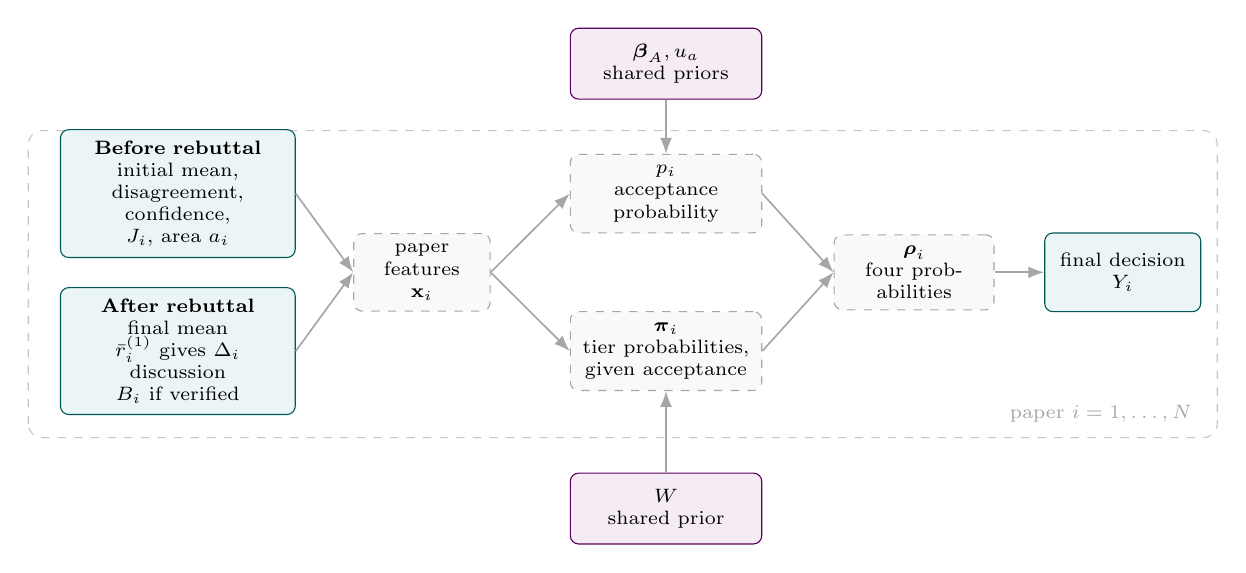
\begin{tikzpicture}[
  >=Latex,
  every node/.style={font=\scriptsize,align=center},
  observed/.style={draw=teal!70!black,rounded corners=3pt,fill=teal!8,minimum height=10mm,inner sep=4pt},
  parameter/.style={draw=violet!70!black,rounded corners=3pt,fill=violet!8,minimum height=9mm,inner sep=4pt},
  deterministic/.style={draw=gray!70,dashed,rounded corners=3pt,fill=gray!5,minimum height=9mm,inner sep=4pt},
  arrow/.style={->,semithick,draw=gray!70}
]
  \draw[gray!45,dashed,rounded corners=5pt] (-0.9,-0.1) rectangle (14.2,3.8);
  \node[observed,text width=2.7cm] (initial) at (1.0,3.0)
    {\textbf{Before rebuttal}\\initial mean, disagreement,\\confidence, $J_i$, area $a_i$};
  \node[observed,text width=2.7cm] (update) at (1.0,1.0)
    {\textbf{After rebuttal}\\final mean $\bar r_i^{(1)}$ gives $\Delta_i$\\discussion $B_i$ if verified};
  \node[deterministic,text width=1.45cm] (features) at (4.1,2.0)
    {paper features\\$\mathbf{x}_i$};
  \node[parameter,text width=2.15cm] (acceptparam) at (7.2,4.65)
    {$\boldsymbol\beta_A,u_a$\\shared priors};
  \node[parameter,text width=2.15cm] (tierparam) at (7.2,-1.0)
    {$W$\\shared prior};
  \node[deterministic,text width=2.15cm] (accept) at (7.2,3.0)
    {$p_i$\\acceptance probability};
  \node[deterministic,text width=2.15cm] (tier) at (7.2,1.0)
    {$\boldsymbol\pi_i$\\tier probabilities,\\given acceptance};
  \node[deterministic,text width=1.75cm] (four) at (10.35,2.0)
    {$\boldsymbol\rho_i$\\four probabilities};
  \node[observed,text width=1.7cm] (decision) at (13.0,2.0)
    {final decision\\$Y_i$};

  \draw[arrow] (initial.east) -- (features.west);
  \draw[arrow] (update.east) -- (features.west);
  \draw[arrow] (features.east) -- (accept.west);
  \draw[arrow] (features.east) -- (tier.west);
  \draw[arrow] (acceptparam.south) -- (accept.north);
  \draw[arrow] (tierparam.north) -- (tier.south);
  \draw[arrow] (accept.east) -- (four.west);
  \draw[arrow] (tier.east) -- (four.west);
  \draw[arrow] (four.east) -- (decision.west);
  \node[anchor=east,text=gray!70] at (14.0,0.2) {paper $i=1,\ldots,N$};
\end{tikzpicture}
\caption{Two-stage conditional graphical model. Teal nodes are observed inputs or outcomes, purple nodes are shared unknown parameters with priors, and dashed nodes are deterministic calculations. The plate repeats for each paper. The model conditions on observed features; it does not model their joint distribution. The discussion feature $B_i$ enters only if verified thread events are available.}
\label{fig:review-model}
\end{figure}

This graph expands $p(Y_i\mid\mathbf{x}_i,\theta)$ into acceptance and presentation-tier stages. Initial ratings may be associated with whether authors reply; the model does not assume the components of $\mathbf{x}_i$ are independent. It conditions on their observed joint values, without fitting $p(\mathbf{x}_i)$ or a paper-specific latent quality variable. The unknown shared parameters comprise acceptance coefficients $\boldsymbol\beta_A$, area effects $u_a$, and tier coefficients $W$. The initial mean $\bar r_i^{(0)}$ and change $\Delta_i$ enter the regression; the final mean is used to compute $\Delta_i$, avoiding three exactly dependent linear predictors.

Let $A_i=1$ if paper $i$ is accepted and $A_i=0$ if it is rejected. A concrete after-rebuttal \emph{likelihood} is
\begin{equation*}
 A_i\sim\operatorname{Bernoulli}(p_i),\qquad
 \operatorname{logit}(p_i)
 =\alpha+\beta_0\bar r_i^{(0)}+\beta_D D_i^{(0)}
  +\beta_c\bar c_i^{(0)}+\beta_J J_i
  +\beta_{\Delta}\Delta_i+\beta_B B_i
  +\beta_{0B}\bar r_i^{(0)}B_i+u_{a(i)}.
\end{equation*}
Here $p_i$ is the acceptance probability, $\bar c_i^{(0)}$ is mean initial confidence, and $u_{a(i)}$ is the unknown effect of research area $a_i$. The interaction permits the predictive association of replies to differ by initial rating. We will include terms involving $B_i$ only if timestamped replies can be verified. H2 is evaluated by comparing posterior predictions at a fixed final mean while changing $\Delta_i$ and setting $\bar r_i^{(0)}=\bar r_i^{(1)}-\Delta_i$ accordingly. H1 and H3 likewise use posterior predictive comparisons at the stated matched initial ratings rather than treating any single coefficient as the entire hypothesis test.

Among accepted papers, let $T_i\in\{P,S,O\}$ denote Poster, Spotlight, or Oral. A second regression gives
\begin{equation*}
 T_i\mid A_i=1,\mathbf{x}_i,W\sim\operatorname{Categorical}(\boldsymbol\pi_i),
 \qquad \boldsymbol\pi_i=\operatorname{softmax}(W\mathbf{z}_i),
\end{equation*}
where $\mathbf{z}_i$ encodes the observed predictors and a constant, with the Poster row of $W$ fixed to zero for identification. The two stages produce
\begin{equation*}
 \boldsymbol\rho_i=\bigl(1-p_i,\ p_i\pi_{i,P},\ p_i\pi_{i,S},\ p_i\pi_{i,O}\bigr),
 \qquad Y_i\mid\mathbf{x}_i,\theta\sim\operatorname{Categorical}(\boldsymbol\rho_i).
\end{equation*}

After standardizing the continuous predictors, one possible set of \emph{priors} is
\begin{equation*}
 \beta_\ell\sim\mathcal{N}(0,1),\quad
 W_{k\ell}\sim\mathcal{N}(0,1)\ (k\in\{S,O\}),\qquad
 \alpha\sim\mathcal{N}(0,2^2),\qquad
 u_a\sim\mathcal{N}(0,\tau^2),\quad
 \tau\sim\operatorname{HalfNormal}(1).
\end{equation*}
These independent coefficient priors are a convenient starting choice; they do \emph{not} assert that the observed predictors are independent. The shared prior on $u_a$ lets areas with little data borrow information from other areas. The acceptance stage learns from every labeled training paper, whereas the tier stage learns from accepted training papers. Updating the priors gives $p(\theta\mid\mathcal D_{\mathrm{train}})$; averaging $\boldsymbol\rho_i$ over posterior draws gives four predictive probabilities for a held-out paper. For an \emph{initial-review} prediction, we will fit a separate version using only initial ratings and confidence; rebuttal changes and replies are unavailable at that time. Reviewer IDs are local to each paper, so we will not try to estimate persistent reviewer strictness across papers.

\section*{Three initial hypotheses}
\begin{enumerate}[label=\textbf{H\arabic*.}]
 \item \textbf{Reviewer disagreement.} Among papers with similar \emph{initial} mean ratings, greater dispersion among reviewers is associated with a higher probability of rejection. This asks whether the distribution of ratings matters beyond their average.
 \item \textbf{Rebuttal trajectory.} Among papers with similar \emph{final} mean ratings, papers whose ratings rose from a lower initial mean have a different probability of acceptance or presentation tier from papers whose ratings remained stable. The direction of this difference is left open because the initial concern and its resolution may carry competing signals.
 \item \textbf{Discussion participation.} Among papers with similar initial ratings and disagreement, papers with both author and reviewer replies during rebuttal have a different final-decision distribution from papers without two-sided participation. This is an observational association, not a claim that replying causes acceptance.
\end{enumerate}

\section*{Planned analysis and evaluation}
We will compare against a mean-rating-only baseline at \emph{the same prediction time}: initial mean versus models using only information available after initial reviews, and final mean versus models using information available after rebuttal but before the decision. Bayesian posterior distributions will quantify uncertainty in the three hypothesized effects and in predicted outcome probabilities. Posterior predictive checks will assess whether the model reproduces observed decision patterns; held-out multiclass log loss, calibration, and class-wise performance will assess predictive value, especially for the relatively rare spotlight and oral classes. Hypotheses may be refined using training data, but the final claims and model comparison will be evaluated on held-out papers. Since this study uses only ICLR 2025, it will assess prediction within that year rather than generalization to future conferences. Because the data are observational, estimated effects will be interpreted as predictive associations rather than causal effects.

\end{document}
